% Created by tikzDevice version 0.12.3 on 2019-09-28 15:41:39
% !TEX encoding = UTF-8 Unicode
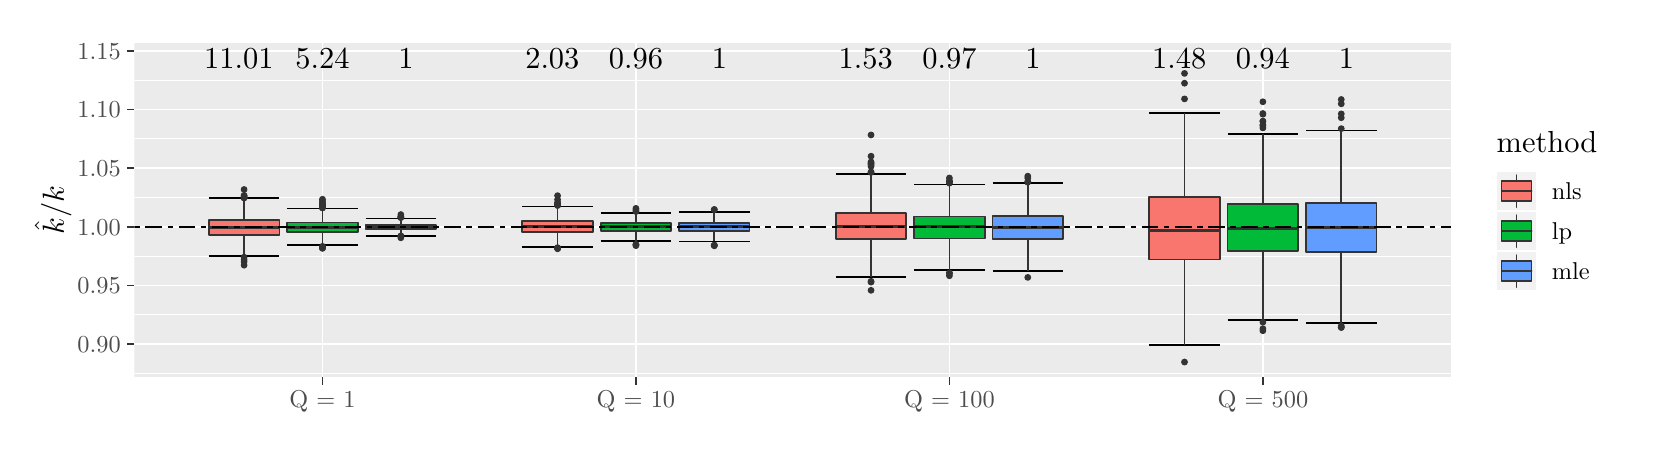
\begin{tikzpicture}[x=1pt,y=1pt]
\definecolor{fillColor}{RGB}{255,255,255}
\path[use as bounding box,fill=fillColor,fill opacity=0.00] (0,0) rectangle (578.16,144.54);
\begin{scope}
\path[clip] (  0.00,  0.00) rectangle (578.16,144.54);
\definecolor{drawColor}{RGB}{255,255,255}
\definecolor{fillColor}{RGB}{255,255,255}

\path[draw=drawColor,line width= 0.6pt,line join=round,line cap=round,fill=fillColor] (  0.00,  0.00) rectangle (578.16,144.54);
\end{scope}
\begin{scope}
\path[clip] ( 38.56, 18.22) rectangle (514.31,139.04);
\definecolor{fillColor}{gray}{0.92}

\path[fill=fillColor] ( 38.56, 18.22) rectangle (514.31,139.04);
\definecolor{drawColor}{RGB}{255,255,255}

\path[draw=drawColor,line width= 0.3pt,line join=round] ( 38.56, 19.64) --
	(514.31, 19.64);

\path[draw=drawColor,line width= 0.3pt,line join=round] ( 38.56, 40.82) --
	(514.31, 40.82);

\path[draw=drawColor,line width= 0.3pt,line join=round] ( 38.56, 62.00) --
	(514.31, 62.00);

\path[draw=drawColor,line width= 0.3pt,line join=round] ( 38.56, 83.18) --
	(514.31, 83.18);

\path[draw=drawColor,line width= 0.3pt,line join=round] ( 38.56,104.36) --
	(514.31,104.36);

\path[draw=drawColor,line width= 0.3pt,line join=round] ( 38.56,125.54) --
	(514.31,125.54);

\path[draw=drawColor,line width= 0.6pt,line join=round] ( 38.56, 30.23) --
	(514.31, 30.23);

\path[draw=drawColor,line width= 0.6pt,line join=round] ( 38.56, 51.41) --
	(514.31, 51.41);

\path[draw=drawColor,line width= 0.6pt,line join=round] ( 38.56, 72.59) --
	(514.31, 72.59);

\path[draw=drawColor,line width= 0.6pt,line join=round] ( 38.56, 93.77) --
	(514.31, 93.77);

\path[draw=drawColor,line width= 0.6pt,line join=round] ( 38.56,114.95) --
	(514.31,114.95);

\path[draw=drawColor,line width= 0.6pt,line join=round] ( 38.56,136.13) --
	(514.31,136.13);

\path[draw=drawColor,line width= 0.6pt,line join=round] (106.52, 18.22) --
	(106.52,139.04);

\path[draw=drawColor,line width= 0.6pt,line join=round] (219.79, 18.22) --
	(219.79,139.04);

\path[draw=drawColor,line width= 0.6pt,line join=round] (333.07, 18.22) --
	(333.07,139.04);

\path[draw=drawColor,line width= 0.6pt,line join=round] (446.34, 18.22) --
	(446.34,139.04);
\definecolor{drawColor}{RGB}{0,0,0}

\path[draw=drawColor,line width= 0.6pt,line join=round] ( 65.46, 82.89) --
	( 90.94, 82.89);

\path[draw=drawColor,line width= 0.6pt,line join=round] ( 78.20, 82.89) --
	( 78.20, 61.95);

\path[draw=drawColor,line width= 0.6pt,line join=round] ( 65.46, 61.95) --
	( 90.94, 61.95);

\path[draw=drawColor,line width= 0.6pt,line join=round] ( 93.78, 79.25) --
	(119.26, 79.25);

\path[draw=drawColor,line width= 0.6pt,line join=round] (106.52, 79.25) --
	(106.52, 66.05);

\path[draw=drawColor,line width= 0.6pt,line join=round] ( 93.78, 66.05) --
	(119.26, 66.05);

\path[draw=drawColor,line width= 0.6pt,line join=round] (122.09, 75.61) --
	(147.58, 75.61);

\path[draw=drawColor,line width= 0.6pt,line join=round] (134.84, 75.61) --
	(134.84, 69.37);

\path[draw=drawColor,line width= 0.6pt,line join=round] (122.09, 69.37) --
	(147.58, 69.37);

\path[draw=drawColor,line width= 0.6pt,line join=round] (178.73, 79.91) --
	(204.22, 79.91);

\path[draw=drawColor,line width= 0.6pt,line join=round] (191.48, 79.91) --
	(191.48, 65.19);

\path[draw=drawColor,line width= 0.6pt,line join=round] (178.73, 65.19) --
	(204.22, 65.19);

\path[draw=drawColor,line width= 0.6pt,line join=round] (207.05, 77.62) --
	(232.54, 77.62);

\path[draw=drawColor,line width= 0.6pt,line join=round] (219.79, 77.62) --
	(219.79, 67.35);

\path[draw=drawColor,line width= 0.6pt,line join=round] (207.05, 67.35) --
	(232.54, 67.35);

\path[draw=drawColor,line width= 0.6pt,line join=round] (235.37, 78.01) --
	(260.86, 78.01);

\path[draw=drawColor,line width= 0.6pt,line join=round] (248.11, 78.01) --
	(248.11, 67.30);

\path[draw=drawColor,line width= 0.6pt,line join=round] (235.37, 67.30) --
	(260.86, 67.30);

\path[draw=drawColor,line width= 0.6pt,line join=round] (292.01, 91.63) --
	(317.49, 91.63);

\path[draw=drawColor,line width= 0.6pt,line join=round] (304.75, 91.63) --
	(304.75, 54.53);

\path[draw=drawColor,line width= 0.6pt,line join=round] (292.01, 54.53) --
	(317.49, 54.53);

\path[draw=drawColor,line width= 0.6pt,line join=round] (320.33, 87.92) --
	(345.81, 87.92);

\path[draw=drawColor,line width= 0.6pt,line join=round] (333.07, 87.92) --
	(333.07, 57.05);

\path[draw=drawColor,line width= 0.6pt,line join=round] (320.33, 57.05) --
	(345.81, 57.05);

\path[draw=drawColor,line width= 0.6pt,line join=round] (348.64, 88.38) --
	(374.13, 88.38);

\path[draw=drawColor,line width= 0.6pt,line join=round] (361.39, 88.38) --
	(361.39, 56.65);

\path[draw=drawColor,line width= 0.6pt,line join=round] (348.64, 56.65) --
	(374.13, 56.65);

\path[draw=drawColor,line width= 0.6pt,line join=round] (405.28,113.69) --
	(430.77,113.69);

\path[draw=drawColor,line width= 0.6pt,line join=round] (418.02,113.69) --
	(418.02, 29.78);

\path[draw=drawColor,line width= 0.6pt,line join=round] (405.28, 29.78) --
	(430.77, 29.78);

\path[draw=drawColor,line width= 0.6pt,line join=round] (433.60,106.06) --
	(459.09,106.06);

\path[draw=drawColor,line width= 0.6pt,line join=round] (446.34,106.06) --
	(446.34, 38.85);

\path[draw=drawColor,line width= 0.6pt,line join=round] (433.60, 38.85) --
	(459.09, 38.85);

\path[draw=drawColor,line width= 0.6pt,line join=round] (461.92,107.44) --
	(487.40,107.44);

\path[draw=drawColor,line width= 0.6pt,line join=round] (474.66,107.44) --
	(474.66, 37.76);

\path[draw=drawColor,line width= 0.6pt,line join=round] (461.92, 37.76) --
	(487.40, 37.76);
\definecolor{drawColor}{gray}{0.20}
\definecolor{fillColor}{gray}{0.20}

\path[draw=drawColor,line width= 0.4pt,line join=round,line cap=round,fill=fillColor] ( 78.20, 58.72) circle (  1.02);

\path[draw=drawColor,line width= 0.4pt,line join=round,line cap=round,fill=fillColor] ( 78.20, 83.11) circle (  1.02);

\path[draw=drawColor,line width= 0.4pt,line join=round,line cap=round,fill=fillColor] ( 78.20, 83.79) circle (  1.02);

\path[draw=drawColor,line width= 0.4pt,line join=round,line cap=round,fill=fillColor] ( 78.20, 83.06) circle (  1.02);

\path[draw=drawColor,line width= 0.4pt,line join=round,line cap=round,fill=fillColor] ( 78.20, 83.40) circle (  1.02);

\path[draw=drawColor,line width= 0.4pt,line join=round,line cap=round,fill=fillColor] ( 78.20, 61.62) circle (  1.02);

\path[draw=drawColor,line width= 0.4pt,line join=round,line cap=round,fill=fillColor] ( 78.20, 86.06) circle (  1.02);

\path[draw=drawColor,line width= 0.4pt,line join=round,line cap=round,fill=fillColor] ( 78.20, 83.05) circle (  1.02);

\path[draw=drawColor,line width= 0.4pt,line join=round,line cap=round,fill=fillColor] ( 78.20, 60.72) circle (  1.02);

\path[draw=drawColor,line width= 0.4pt,line join=round,line cap=round,fill=fillColor] ( 78.20, 59.94) circle (  1.02);

\path[draw=drawColor,line width= 0.4pt,line join=round,line cap=round,fill=fillColor] ( 78.20, 83.92) circle (  1.02);

\path[draw=drawColor,line width= 0.6pt,line join=round] ( 78.20, 75.01) -- ( 78.20, 82.89);

\path[draw=drawColor,line width= 0.6pt,line join=round] ( 78.20, 69.73) -- ( 78.20, 61.95);
\definecolor{fillColor}{RGB}{248,118,109}

\path[draw=drawColor,line width= 0.6pt,line join=round,line cap=round,fill=fillColor] ( 65.46, 75.01) --
	( 65.46, 69.73) --
	( 90.94, 69.73) --
	( 90.94, 75.01) --
	( 65.46, 75.01) --
	cycle;

\path[draw=drawColor,line width= 1.1pt,line join=round] ( 65.46, 72.35) -- ( 90.94, 72.35);
\definecolor{fillColor}{gray}{0.20}

\path[draw=drawColor,line width= 0.4pt,line join=round,line cap=round,fill=fillColor] (106.52, 79.83) circle (  1.02);

\path[draw=drawColor,line width= 0.4pt,line join=round,line cap=round,fill=fillColor] (106.52, 79.53) circle (  1.02);

\path[draw=drawColor,line width= 0.4pt,line join=round,line cap=round,fill=fillColor] (106.52, 64.90) circle (  1.02);

\path[draw=drawColor,line width= 0.4pt,line join=round,line cap=round,fill=fillColor] (106.52, 64.83) circle (  1.02);

\path[draw=drawColor,line width= 0.4pt,line join=round,line cap=round,fill=fillColor] (106.52, 81.94) circle (  1.02);

\path[draw=drawColor,line width= 0.4pt,line join=round,line cap=round,fill=fillColor] (106.52, 79.39) circle (  1.02);

\path[draw=drawColor,line width= 0.4pt,line join=round,line cap=round,fill=fillColor] (106.52, 79.97) circle (  1.02);

\path[draw=drawColor,line width= 0.4pt,line join=round,line cap=round,fill=fillColor] (106.52, 81.14) circle (  1.02);

\path[draw=drawColor,line width= 0.4pt,line join=round,line cap=round,fill=fillColor] (106.52, 79.55) circle (  1.02);

\path[draw=drawColor,line width= 0.4pt,line join=round,line cap=round,fill=fillColor] (106.52, 65.51) circle (  1.02);

\path[draw=drawColor,line width= 0.4pt,line join=round,line cap=round,fill=fillColor] (106.52, 79.69) circle (  1.02);

\path[draw=drawColor,line width= 0.4pt,line join=round,line cap=round,fill=fillColor] (106.52, 80.25) circle (  1.02);

\path[draw=drawColor,line width= 0.4pt,line join=round,line cap=round,fill=fillColor] (106.52, 80.32) circle (  1.02);

\path[draw=drawColor,line width= 0.4pt,line join=round,line cap=round,fill=fillColor] (106.52, 81.14) circle (  1.02);

\path[draw=drawColor,line width= 0.4pt,line join=round,line cap=round,fill=fillColor] (106.52, 80.74) circle (  1.02);

\path[draw=drawColor,line width= 0.4pt,line join=round,line cap=round,fill=fillColor] (106.52, 82.53) circle (  1.02);

\path[draw=drawColor,line width= 0.4pt,line join=round,line cap=round,fill=fillColor] (106.52, 65.22) circle (  1.02);

\path[draw=drawColor,line width= 0.4pt,line join=round,line cap=round,fill=fillColor] (106.52, 65.33) circle (  1.02);

\path[draw=drawColor,line width= 0.4pt,line join=round,line cap=round,fill=fillColor] (106.52, 64.92) circle (  1.02);

\path[draw=drawColor,line width= 0.6pt,line join=round] (106.52, 74.17) -- (106.52, 79.25);

\path[draw=drawColor,line width= 0.6pt,line join=round] (106.52, 70.73) -- (106.52, 66.05);
\definecolor{fillColor}{RGB}{0,186,56}

\path[draw=drawColor,line width= 0.6pt,line join=round,line cap=round,fill=fillColor] ( 93.78, 74.17) --
	( 93.78, 70.73) --
	(119.26, 70.73) --
	(119.26, 74.17) --
	( 93.78, 74.17) --
	cycle;

\path[draw=drawColor,line width= 1.1pt,line join=round] ( 93.78, 72.49) -- (119.26, 72.49);
\definecolor{fillColor}{gray}{0.20}

\path[draw=drawColor,line width= 0.4pt,line join=round,line cap=round,fill=fillColor] (134.84, 76.16) circle (  1.02);

\path[draw=drawColor,line width= 0.4pt,line join=round,line cap=round,fill=fillColor] (134.84, 77.00) circle (  1.02);

\path[draw=drawColor,line width= 0.4pt,line join=round,line cap=round,fill=fillColor] (134.84, 75.89) circle (  1.02);

\path[draw=drawColor,line width= 0.4pt,line join=round,line cap=round,fill=fillColor] (134.84, 76.28) circle (  1.02);

\path[draw=drawColor,line width= 0.4pt,line join=round,line cap=round,fill=fillColor] (134.84, 69.27) circle (  1.02);

\path[draw=drawColor,line width= 0.4pt,line join=round,line cap=round,fill=fillColor] (134.84, 68.61) circle (  1.02);

\path[draw=drawColor,line width= 0.4pt,line join=round,line cap=round,fill=fillColor] (134.84, 69.18) circle (  1.02);

\path[draw=drawColor,line width= 0.4pt,line join=round,line cap=round,fill=fillColor] (134.84, 76.06) circle (  1.02);

\path[draw=drawColor,line width= 0.6pt,line join=round] (134.84, 73.26) -- (134.84, 75.61);

\path[draw=drawColor,line width= 0.6pt,line join=round] (134.84, 71.67) -- (134.84, 69.37);
\definecolor{fillColor}{RGB}{97,156,255}

\path[draw=drawColor,line width= 0.6pt,line join=round,line cap=round,fill=fillColor] (122.09, 73.26) --
	(122.09, 71.67) --
	(147.58, 71.67) --
	(147.58, 73.26) --
	(122.09, 73.26) --
	cycle;

\path[draw=drawColor,line width= 1.1pt,line join=round] (122.09, 72.44) -- (147.58, 72.44);
\definecolor{fillColor}{gray}{0.20}

\path[draw=drawColor,line width= 0.4pt,line join=round,line cap=round,fill=fillColor] (191.48, 80.48) circle (  1.02);

\path[draw=drawColor,line width= 0.4pt,line join=round,line cap=round,fill=fillColor] (191.48, 64.85) circle (  1.02);

\path[draw=drawColor,line width= 0.4pt,line join=round,line cap=round,fill=fillColor] (191.48, 83.84) circle (  1.02);

\path[draw=drawColor,line width= 0.4pt,line join=round,line cap=round,fill=fillColor] (191.48, 80.62) circle (  1.02);

\path[draw=drawColor,line width= 0.4pt,line join=round,line cap=round,fill=fillColor] (191.48, 64.65) circle (  1.02);

\path[draw=drawColor,line width= 0.4pt,line join=round,line cap=round,fill=fillColor] (191.48, 64.88) circle (  1.02);

\path[draw=drawColor,line width= 0.4pt,line join=round,line cap=round,fill=fillColor] (191.48, 64.97) circle (  1.02);

\path[draw=drawColor,line width= 0.4pt,line join=round,line cap=round,fill=fillColor] (191.48, 82.42) circle (  1.02);

\path[draw=drawColor,line width= 0.4pt,line join=round,line cap=round,fill=fillColor] (191.48, 81.42) circle (  1.02);

\path[draw=drawColor,line width= 0.4pt,line join=round,line cap=round,fill=fillColor] (191.48, 80.92) circle (  1.02);

\path[draw=drawColor,line width= 0.4pt,line join=round,line cap=round,fill=fillColor] (191.48, 80.30) circle (  1.02);

\path[draw=drawColor,line width= 0.4pt,line join=round,line cap=round,fill=fillColor] (191.48, 80.36) circle (  1.02);

\path[draw=drawColor,line width= 0.4pt,line join=round,line cap=round,fill=fillColor] (191.48, 64.99) circle (  1.02);

\path[draw=drawColor,line width= 0.6pt,line join=round] (191.48, 74.57) -- (191.48, 79.91);

\path[draw=drawColor,line width= 0.6pt,line join=round] (191.48, 70.78) -- (191.48, 65.19);
\definecolor{fillColor}{RGB}{248,118,109}

\path[draw=drawColor,line width= 0.6pt,line join=round,line cap=round,fill=fillColor] (178.73, 74.57) --
	(178.73, 70.78) --
	(204.22, 70.78) --
	(204.22, 74.57) --
	(178.73, 74.57) --
	cycle;

\path[draw=drawColor,line width= 1.1pt,line join=round] (178.73, 72.52) -- (204.22, 72.52);
\definecolor{fillColor}{gray}{0.20}

\path[draw=drawColor,line width= 0.4pt,line join=round,line cap=round,fill=fillColor] (219.79, 66.18) circle (  1.02);

\path[draw=drawColor,line width= 0.4pt,line join=round,line cap=round,fill=fillColor] (219.79, 66.20) circle (  1.02);

\path[draw=drawColor,line width= 0.4pt,line join=round,line cap=round,fill=fillColor] (219.79, 65.77) circle (  1.02);

\path[draw=drawColor,line width= 0.4pt,line join=round,line cap=round,fill=fillColor] (219.79, 78.10) circle (  1.02);

\path[draw=drawColor,line width= 0.4pt,line join=round,line cap=round,fill=fillColor] (219.79, 79.25) circle (  1.02);

\path[draw=drawColor,line width= 0.4pt,line join=round,line cap=round,fill=fillColor] (219.79, 78.65) circle (  1.02);

\path[draw=drawColor,line width= 0.6pt,line join=round] (219.79, 73.90) -- (219.79, 77.62);

\path[draw=drawColor,line width= 0.6pt,line join=round] (219.79, 71.15) -- (219.79, 67.35);
\definecolor{fillColor}{RGB}{0,186,56}

\path[draw=drawColor,line width= 0.6pt,line join=round,line cap=round,fill=fillColor] (207.05, 73.90) --
	(207.05, 71.15) --
	(232.54, 71.15) --
	(232.54, 73.90) --
	(207.05, 73.90) --
	cycle;

\path[draw=drawColor,line width= 1.1pt,line join=round] (207.05, 72.52) -- (232.54, 72.52);
\definecolor{fillColor}{gray}{0.20}

\path[draw=drawColor,line width= 0.4pt,line join=round,line cap=round,fill=fillColor] (248.11, 65.93) circle (  1.02);

\path[draw=drawColor,line width= 0.4pt,line join=round,line cap=round,fill=fillColor] (248.11, 65.92) circle (  1.02);

\path[draw=drawColor,line width= 0.4pt,line join=round,line cap=round,fill=fillColor] (248.11, 65.72) circle (  1.02);

\path[draw=drawColor,line width= 0.4pt,line join=round,line cap=round,fill=fillColor] (248.11, 78.80) circle (  1.02);

\path[draw=drawColor,line width= 0.4pt,line join=round,line cap=round,fill=fillColor] (248.11, 78.82) circle (  1.02);

\path[draw=drawColor,line width= 0.6pt,line join=round] (248.11, 73.93) -- (248.11, 78.01);

\path[draw=drawColor,line width= 0.6pt,line join=round] (248.11, 71.15) -- (248.11, 67.30);
\definecolor{fillColor}{RGB}{97,156,255}

\path[draw=drawColor,line width= 0.6pt,line join=round,line cap=round,fill=fillColor] (235.37, 73.93) --
	(235.37, 71.15) --
	(260.86, 71.15) --
	(260.86, 73.93) --
	(235.37, 73.93) --
	cycle;

\path[draw=drawColor,line width= 1.1pt,line join=round] (235.37, 72.58) -- (260.86, 72.58);
\definecolor{fillColor}{gray}{0.20}

\path[draw=drawColor,line width= 0.4pt,line join=round,line cap=round,fill=fillColor] (304.75, 95.30) circle (  1.02);

\path[draw=drawColor,line width= 0.4pt,line join=round,line cap=round,fill=fillColor] (304.75, 96.02) circle (  1.02);

\path[draw=drawColor,line width= 0.4pt,line join=round,line cap=round,fill=fillColor] (304.75, 92.24) circle (  1.02);

\path[draw=drawColor,line width= 0.4pt,line join=round,line cap=round,fill=fillColor] (304.75, 52.89) circle (  1.02);

\path[draw=drawColor,line width= 0.4pt,line join=round,line cap=round,fill=fillColor] (304.75,105.77) circle (  1.02);

\path[draw=drawColor,line width= 0.4pt,line join=round,line cap=round,fill=fillColor] (304.75, 98.09) circle (  1.02);

\path[draw=drawColor,line width= 0.4pt,line join=round,line cap=round,fill=fillColor] (304.75, 92.39) circle (  1.02);

\path[draw=drawColor,line width= 0.4pt,line join=round,line cap=round,fill=fillColor] (304.75, 49.63) circle (  1.02);

\path[draw=drawColor,line width= 0.4pt,line join=round,line cap=round,fill=fillColor] (304.75, 94.97) circle (  1.02);

\path[draw=drawColor,line width= 0.4pt,line join=round,line cap=round,fill=fillColor] (304.75, 94.41) circle (  1.02);

\path[draw=drawColor,line width= 0.4pt,line join=round,line cap=round,fill=fillColor] (304.75, 52.58) circle (  1.02);

\path[draw=drawColor,line width= 0.4pt,line join=round,line cap=round,fill=fillColor] (304.75, 95.69) circle (  1.02);

\path[draw=drawColor,line width= 0.6pt,line join=round] (304.75, 77.68) -- (304.75, 91.63);

\path[draw=drawColor,line width= 0.6pt,line join=round] (304.75, 68.10) -- (304.75, 54.53);
\definecolor{fillColor}{RGB}{248,118,109}

\path[draw=drawColor,line width= 0.6pt,line join=round,line cap=round,fill=fillColor] (292.01, 77.68) --
	(292.01, 68.10) --
	(317.49, 68.10) --
	(317.49, 77.68) --
	(292.01, 77.68) --
	cycle;

\path[draw=drawColor,line width= 1.1pt,line join=round] (292.01, 72.84) -- (317.49, 72.84);
\definecolor{fillColor}{gray}{0.20}

\path[draw=drawColor,line width= 0.4pt,line join=round,line cap=round,fill=fillColor] (333.07, 55.96) circle (  1.02);

\path[draw=drawColor,line width= 0.4pt,line join=round,line cap=round,fill=fillColor] (333.07, 88.84) circle (  1.02);

\path[draw=drawColor,line width= 0.4pt,line join=round,line cap=round,fill=fillColor] (333.07, 90.22) circle (  1.02);

\path[draw=drawColor,line width= 0.4pt,line join=round,line cap=round,fill=fillColor] (333.07, 89.22) circle (  1.02);

\path[draw=drawColor,line width= 0.4pt,line join=round,line cap=round,fill=fillColor] (333.07, 55.74) circle (  1.02);

\path[draw=drawColor,line width= 0.4pt,line join=round,line cap=round,fill=fillColor] (333.07, 54.90) circle (  1.02);

\path[draw=drawColor,line width= 0.4pt,line join=round,line cap=round,fill=fillColor] (333.07, 88.85) circle (  1.02);

\path[draw=drawColor,line width= 0.4pt,line join=round,line cap=round,fill=fillColor] (333.07, 88.35) circle (  1.02);

\path[draw=drawColor,line width= 0.6pt,line join=round] (333.07, 76.25) -- (333.07, 87.92);

\path[draw=drawColor,line width= 0.6pt,line join=round] (333.07, 68.38) -- (333.07, 57.05);
\definecolor{fillColor}{RGB}{0,186,56}

\path[draw=drawColor,line width= 0.6pt,line join=round,line cap=round,fill=fillColor] (320.33, 76.25) --
	(320.33, 68.38) --
	(345.81, 68.38) --
	(345.81, 76.25) --
	(320.33, 76.25) --
	cycle;

\path[draw=drawColor,line width= 1.1pt,line join=round] (320.33, 72.64) -- (345.81, 72.64);
\definecolor{fillColor}{gray}{0.20}

\path[draw=drawColor,line width= 0.4pt,line join=round,line cap=round,fill=fillColor] (361.39, 90.89) circle (  1.02);

\path[draw=drawColor,line width= 0.4pt,line join=round,line cap=round,fill=fillColor] (361.39, 90.19) circle (  1.02);

\path[draw=drawColor,line width= 0.4pt,line join=round,line cap=round,fill=fillColor] (361.39, 54.30) circle (  1.02);

\path[draw=drawColor,line width= 0.4pt,line join=round,line cap=round,fill=fillColor] (361.39, 88.90) circle (  1.02);

\path[draw=drawColor,line width= 0.4pt,line join=round,line cap=round,fill=fillColor] (361.39, 88.70) circle (  1.02);

\path[draw=drawColor,line width= 0.6pt,line join=round] (361.39, 76.42) -- (361.39, 88.38);

\path[draw=drawColor,line width= 0.6pt,line join=round] (361.39, 68.25) -- (361.39, 56.65);
\definecolor{fillColor}{RGB}{97,156,255}

\path[draw=drawColor,line width= 0.6pt,line join=round,line cap=round,fill=fillColor] (348.64, 76.42) --
	(348.64, 68.25) --
	(374.13, 68.25) --
	(374.13, 76.42) --
	(348.64, 76.42) --
	cycle;

\path[draw=drawColor,line width= 1.1pt,line join=round] (348.64, 72.45) -- (374.13, 72.45);
\definecolor{fillColor}{gray}{0.20}

\path[draw=drawColor,line width= 0.4pt,line join=round,line cap=round,fill=fillColor] (418.02,128.01) circle (  1.02);

\path[draw=drawColor,line width= 0.4pt,line join=round,line cap=round,fill=fillColor] (418.02,124.47) circle (  1.02);

\path[draw=drawColor,line width= 0.4pt,line join=round,line cap=round,fill=fillColor] (418.02, 23.71) circle (  1.02);

\path[draw=drawColor,line width= 0.4pt,line join=round,line cap=round,fill=fillColor] (418.02,118.80) circle (  1.02);

\path[draw=drawColor,line width= 0.6pt,line join=round] (418.02, 83.28) -- (418.02,113.69);

\path[draw=drawColor,line width= 0.6pt,line join=round] (418.02, 60.79) -- (418.02, 29.78);
\definecolor{fillColor}{RGB}{248,118,109}

\path[draw=drawColor,line width= 0.6pt,line join=round,line cap=round,fill=fillColor] (405.28, 83.28) --
	(405.28, 60.79) --
	(430.77, 60.79) --
	(430.77, 83.28) --
	(405.28, 83.28) --
	cycle;

\path[draw=drawColor,line width= 1.1pt,line join=round] (405.28, 71.39) -- (430.77, 71.39);
\definecolor{fillColor}{gray}{0.20}

\path[draw=drawColor,line width= 0.4pt,line join=round,line cap=round,fill=fillColor] (446.34,109.14) circle (  1.02);

\path[draw=drawColor,line width= 0.4pt,line join=round,line cap=round,fill=fillColor] (446.34,117.76) circle (  1.02);

\path[draw=drawColor,line width= 0.4pt,line join=round,line cap=round,fill=fillColor] (446.34,108.31) circle (  1.02);

\path[draw=drawColor,line width= 0.4pt,line join=round,line cap=round,fill=fillColor] (446.34,113.26) circle (  1.02);

\path[draw=drawColor,line width= 0.4pt,line join=round,line cap=round,fill=fillColor] (446.34, 35.76) circle (  1.02);

\path[draw=drawColor,line width= 0.4pt,line join=round,line cap=round,fill=fillColor] (446.34,113.52) circle (  1.02);

\path[draw=drawColor,line width= 0.4pt,line join=round,line cap=round,fill=fillColor] (446.34,110.76) circle (  1.02);

\path[draw=drawColor,line width= 0.4pt,line join=round,line cap=round,fill=fillColor] (446.34, 35.04) circle (  1.02);

\path[draw=drawColor,line width= 0.4pt,line join=round,line cap=round,fill=fillColor] (446.34,109.38) circle (  1.02);

\path[draw=drawColor,line width= 0.4pt,line join=round,line cap=round,fill=fillColor] (446.34, 38.12) circle (  1.02);

\path[draw=drawColor,line width= 0.4pt,line join=round,line cap=round,fill=fillColor] (446.34,110.67) circle (  1.02);

\path[draw=drawColor,line width= 0.6pt,line join=round] (446.34, 80.74) -- (446.34,106.06);

\path[draw=drawColor,line width= 0.6pt,line join=round] (446.34, 63.83) -- (446.34, 38.85);
\definecolor{fillColor}{RGB}{0,186,56}

\path[draw=drawColor,line width= 0.6pt,line join=round,line cap=round,fill=fillColor] (433.60, 80.74) --
	(433.60, 63.83) --
	(459.09, 63.83) --
	(459.09, 80.74) --
	(433.60, 80.74) --
	cycle;

\path[draw=drawColor,line width= 1.1pt,line join=round] (433.60, 71.96) -- (459.09, 71.96);
\definecolor{fillColor}{gray}{0.20}

\path[draw=drawColor,line width= 0.4pt,line join=round,line cap=round,fill=fillColor] (474.66,118.59) circle (  1.02);

\path[draw=drawColor,line width= 0.4pt,line join=round,line cap=round,fill=fillColor] (474.66,113.38) circle (  1.02);

\path[draw=drawColor,line width= 0.4pt,line join=round,line cap=round,fill=fillColor] (474.66,108.05) circle (  1.02);

\path[draw=drawColor,line width= 0.4pt,line join=round,line cap=round,fill=fillColor] (474.66,117.03) circle (  1.02);

\path[draw=drawColor,line width= 0.4pt,line join=round,line cap=round,fill=fillColor] (474.66, 36.20) circle (  1.02);

\path[draw=drawColor,line width= 0.4pt,line join=round,line cap=round,fill=fillColor] (474.66, 36.28) circle (  1.02);

\path[draw=drawColor,line width= 0.4pt,line join=round,line cap=round,fill=fillColor] (474.66, 36.77) circle (  1.02);

\path[draw=drawColor,line width= 0.4pt,line join=round,line cap=round,fill=fillColor] (474.66,112.00) circle (  1.02);

\path[draw=drawColor,line width= 0.6pt,line join=round] (474.66, 81.16) -- (474.66,107.44);

\path[draw=drawColor,line width= 0.6pt,line join=round] (474.66, 63.59) -- (474.66, 37.76);
\definecolor{fillColor}{RGB}{97,156,255}

\path[draw=drawColor,line width= 0.6pt,line join=round,line cap=round,fill=fillColor] (461.92, 81.16) --
	(461.92, 63.59) --
	(487.40, 63.59) --
	(487.40, 81.16) --
	(461.92, 81.16) --
	cycle;

\path[draw=drawColor,line width= 1.1pt,line join=round] (461.92, 72.47) -- (487.40, 72.47);
\definecolor{drawColor}{RGB}{0,0,0}

\path[draw=drawColor,line width= 0.6pt,dash pattern=on 2pt off 2pt on 6pt off 2pt ,line join=round] ( 38.56, 72.59) -- (514.31, 72.59);

\node[text=drawColor,anchor=base,inner sep=0pt, outer sep=0pt, scale=  1.10] at (136.73,129.75) {1};

\node[text=drawColor,anchor=base,inner sep=0pt, outer sep=0pt, scale=  1.10] at (106.52,129.75) {5.24};

\node[text=drawColor,anchor=base,inner sep=0pt, outer sep=0pt, scale=  1.10] at ( 76.31,129.75) {11.01};

\node[text=drawColor,anchor=base,inner sep=0pt, outer sep=0pt, scale=  1.10] at (250.00,129.75) {1};

\node[text=drawColor,anchor=base,inner sep=0pt, outer sep=0pt, scale=  1.10] at (219.79,129.75) {0.96};

\node[text=drawColor,anchor=base,inner sep=0pt, outer sep=0pt, scale=  1.10] at (189.59,129.75) {2.03};

\node[text=drawColor,anchor=base,inner sep=0pt, outer sep=0pt, scale=  1.10] at (363.28,129.75) {1};

\node[text=drawColor,anchor=base,inner sep=0pt, outer sep=0pt, scale=  1.10] at (333.07,129.75) {0.97};

\node[text=drawColor,anchor=base,inner sep=0pt, outer sep=0pt, scale=  1.10] at (302.86,129.75) {1.53};

\node[text=drawColor,anchor=base,inner sep=0pt, outer sep=0pt, scale=  1.10] at (476.55,129.75) {1};

\node[text=drawColor,anchor=base,inner sep=0pt, outer sep=0pt, scale=  1.10] at (446.34,129.75) {0.94};

\node[text=drawColor,anchor=base,inner sep=0pt, outer sep=0pt, scale=  1.10] at (416.14,129.75) {1.48};
\end{scope}
\begin{scope}
\path[clip] (  0.00,  0.00) rectangle (578.16,144.54);
\definecolor{drawColor}{gray}{0.30}

\node[text=drawColor,anchor=base east,inner sep=0pt, outer sep=0pt, scale=  0.88] at ( 33.61, 27.20) {0.90};

\node[text=drawColor,anchor=base east,inner sep=0pt, outer sep=0pt, scale=  0.88] at ( 33.61, 48.38) {0.95};

\node[text=drawColor,anchor=base east,inner sep=0pt, outer sep=0pt, scale=  0.88] at ( 33.61, 69.56) {1.00};

\node[text=drawColor,anchor=base east,inner sep=0pt, outer sep=0pt, scale=  0.88] at ( 33.61, 90.74) {1.05};

\node[text=drawColor,anchor=base east,inner sep=0pt, outer sep=0pt, scale=  0.88] at ( 33.61,111.92) {1.10};

\node[text=drawColor,anchor=base east,inner sep=0pt, outer sep=0pt, scale=  0.88] at ( 33.61,133.10) {1.15};
\end{scope}
\begin{scope}
\path[clip] (  0.00,  0.00) rectangle (578.16,144.54);
\definecolor{drawColor}{gray}{0.20}

\path[draw=drawColor,line width= 0.6pt,line join=round] ( 35.81, 30.23) --
	( 38.56, 30.23);

\path[draw=drawColor,line width= 0.6pt,line join=round] ( 35.81, 51.41) --
	( 38.56, 51.41);

\path[draw=drawColor,line width= 0.6pt,line join=round] ( 35.81, 72.59) --
	( 38.56, 72.59);

\path[draw=drawColor,line width= 0.6pt,line join=round] ( 35.81, 93.77) --
	( 38.56, 93.77);

\path[draw=drawColor,line width= 0.6pt,line join=round] ( 35.81,114.95) --
	( 38.56,114.95);

\path[draw=drawColor,line width= 0.6pt,line join=round] ( 35.81,136.13) --
	( 38.56,136.13);
\end{scope}
\begin{scope}
\path[clip] (  0.00,  0.00) rectangle (578.16,144.54);
\definecolor{drawColor}{gray}{0.20}

\path[draw=drawColor,line width= 0.6pt,line join=round] (106.52, 15.47) --
	(106.52, 18.22);

\path[draw=drawColor,line width= 0.6pt,line join=round] (219.79, 15.47) --
	(219.79, 18.22);

\path[draw=drawColor,line width= 0.6pt,line join=round] (333.07, 15.47) --
	(333.07, 18.22);

\path[draw=drawColor,line width= 0.6pt,line join=round] (446.34, 15.47) --
	(446.34, 18.22);
\end{scope}
\begin{scope}
\path[clip] (  0.00,  0.00) rectangle (578.16,144.54);
\definecolor{drawColor}{gray}{0.30}

\node[text=drawColor,anchor=base,inner sep=0pt, outer sep=0pt, scale=  0.88] at (106.52,  7.21) {Q = 1};

\node[text=drawColor,anchor=base,inner sep=0pt, outer sep=0pt, scale=  0.88] at (219.79,  7.21) {Q = 10};

\node[text=drawColor,anchor=base,inner sep=0pt, outer sep=0pt, scale=  0.88] at (333.07,  7.21) {Q = 100};

\node[text=drawColor,anchor=base,inner sep=0pt, outer sep=0pt, scale=  0.88] at (446.34,  7.21) {Q = 500};
\end{scope}
\begin{scope}
\path[clip] (  0.00,  0.00) rectangle (578.16,144.54);
\definecolor{drawColor}{RGB}{0,0,0}

\node[text=drawColor,rotate= 90.00,anchor=base,inner sep=0pt, outer sep=0pt, scale=  1.10] at ( 13.08, 78.63) {$\hat{k}/k$};
\end{scope}
\begin{scope}
\path[clip] (  0.00,  0.00) rectangle (578.16,144.54);
\definecolor{fillColor}{RGB}{255,255,255}

\path[fill=fillColor] (525.31, 43.84) rectangle (572.66,113.42);
\end{scope}
\begin{scope}
\path[clip] (  0.00,  0.00) rectangle (578.16,144.54);
\definecolor{drawColor}{RGB}{0,0,0}

\node[text=drawColor,anchor=base west,inner sep=0pt, outer sep=0pt, scale=  1.10] at (530.81, 99.27) {method};
\end{scope}
\begin{scope}
\path[clip] (  0.00,  0.00) rectangle (578.16,144.54);
\definecolor{drawColor}{RGB}{255,255,255}
\definecolor{fillColor}{gray}{0.95}

\path[draw=drawColor,line width= 0.6pt,line join=round,line cap=round,fill=fillColor] (530.81, 78.25) rectangle (545.26, 92.70);
\end{scope}
\begin{scope}
\path[clip] (  0.00,  0.00) rectangle (578.16,144.54);
\definecolor{drawColor}{gray}{0.20}

\path[draw=drawColor,line width= 0.6pt,line join=round,line cap=round] (538.03, 79.70) --
	(538.03, 81.86);

\path[draw=drawColor,line width= 0.6pt,line join=round,line cap=round] (538.03, 89.09) --
	(538.03, 91.26);
\definecolor{fillColor}{RGB}{248,118,109}

\path[draw=drawColor,line width= 0.6pt,line join=round,line cap=round,fill=fillColor] (532.61, 81.86) rectangle (543.45, 89.09);

\path[draw=drawColor,line width= 0.6pt,line join=round,line cap=round] (532.61, 85.48) --
	(543.45, 85.48);
\end{scope}
\begin{scope}
\path[clip] (  0.00,  0.00) rectangle (578.16,144.54);
\definecolor{drawColor}{RGB}{255,255,255}
\definecolor{fillColor}{gray}{0.95}

\path[draw=drawColor,line width= 0.6pt,line join=round,line cap=round,fill=fillColor] (530.81, 63.80) rectangle (545.26, 78.25);
\end{scope}
\begin{scope}
\path[clip] (  0.00,  0.00) rectangle (578.16,144.54);
\definecolor{drawColor}{gray}{0.20}

\path[draw=drawColor,line width= 0.6pt,line join=round,line cap=round] (538.03, 65.24) --
	(538.03, 67.41);

\path[draw=drawColor,line width= 0.6pt,line join=round,line cap=round] (538.03, 74.64) --
	(538.03, 76.81);
\definecolor{fillColor}{RGB}{0,186,56}

\path[draw=drawColor,line width= 0.6pt,line join=round,line cap=round,fill=fillColor] (532.61, 67.41) rectangle (543.45, 74.64);

\path[draw=drawColor,line width= 0.6pt,line join=round,line cap=round] (532.61, 71.02) --
	(543.45, 71.02);
\end{scope}
\begin{scope}
\path[clip] (  0.00,  0.00) rectangle (578.16,144.54);
\definecolor{drawColor}{RGB}{255,255,255}
\definecolor{fillColor}{gray}{0.95}

\path[draw=drawColor,line width= 0.6pt,line join=round,line cap=round,fill=fillColor] (530.81, 49.34) rectangle (545.26, 63.80);
\end{scope}
\begin{scope}
\path[clip] (  0.00,  0.00) rectangle (578.16,144.54);
\definecolor{drawColor}{gray}{0.20}

\path[draw=drawColor,line width= 0.6pt,line join=round,line cap=round] (538.03, 50.79) --
	(538.03, 52.96);

\path[draw=drawColor,line width= 0.6pt,line join=round,line cap=round] (538.03, 60.18) --
	(538.03, 62.35);
\definecolor{fillColor}{RGB}{97,156,255}

\path[draw=drawColor,line width= 0.6pt,line join=round,line cap=round,fill=fillColor] (532.61, 52.96) rectangle (543.45, 60.18);

\path[draw=drawColor,line width= 0.6pt,line join=round,line cap=round] (532.61, 56.57) --
	(543.45, 56.57);
\end{scope}
\begin{scope}
\path[clip] (  0.00,  0.00) rectangle (578.16,144.54);
\definecolor{drawColor}{RGB}{0,0,0}

\node[text=drawColor,anchor=base west,inner sep=0pt, outer sep=0pt, scale=  0.88] at (550.76, 82.45) {nls};
\end{scope}
\begin{scope}
\path[clip] (  0.00,  0.00) rectangle (578.16,144.54);
\definecolor{drawColor}{RGB}{0,0,0}

\node[text=drawColor,anchor=base west,inner sep=0pt, outer sep=0pt, scale=  0.88] at (550.76, 67.99) {lp};
\end{scope}
\begin{scope}
\path[clip] (  0.00,  0.00) rectangle (578.16,144.54);
\definecolor{drawColor}{RGB}{0,0,0}

\node[text=drawColor,anchor=base west,inner sep=0pt, outer sep=0pt, scale=  0.88] at (550.76, 53.54) {mle};
\end{scope}
\end{tikzpicture}
